\documentclass[1_relazione.tex]{subfiles}
\begin{document}

\section{Realizzazione}
Questa sezione illustra i passi per la realizzazione di FRENT.  I criteri che abbiamo utilizzato sono:
\begin{itemize}
\item Separazione fra struttura, presentazione e comportamento;
\item Garantire l'accessibilit\`{a};
\item Scelta della corretta tecnologia da impiegare.
\end{itemize}

\subsection{Base di dati}
La base di dati \`{e} stata la prima parte del progetto codificata. A partire dallo schemi ER abbiamo creato le entit\`{a} e le relazioni in SQL. Abbiamo controllato con attenzione le politiche di reazione in caso di cancellazione e modifiche ai dati, in modo che la base di dati fosse sempre coerente. Inoltre abbiamo deciso di implementare tutte le funzionalit\`{a} di base offerte dal sito come funzioni e procedure SQL.

\subsection{Struttura}
Il punto di partenza per la creazione del sito sono state le pagine statiche. In tutte le pagine abbiamo prestato attenzione ai tag utilizzati e a rispettarne il significato semantico come visto in classe e nei laboratori. Abbiamo deciso di implementare le pagine in XHTML e utilizzare HTML5 solo per quelle pagine in cui era indispensabile.\\ Una componente fondamentale per il funzionamento del sito sono le date, un guest deve sempre indicare la data di inizio e di fine di una prenotazione. Per facilitare l'inserimento di questo dato abbiamo scelto di utilizzare il widget-calendario offerto dalla maggior parte dei browser quando è richiesta una data. Abbiamo giudicato improponibile chiedere al guest di inserire 6 numeri (in un formato specifico per giunta) per ogni ricerca. Le pagine di home, elenco risultati e dettagli annunci sono perci\`{o} implementate con HTML5. \\
Abbiamo inoltre implementato gli schemi esatti che sono stati introdotti nella sezione di progettazione realizzati sotto forma di liste. In questa fase abbiamo realizzato gli header e i footer che poi sarebbero stati scelti dinamicamente in un secondo momento. \\
%Per ragioni di accessibilit\`{a}, tutti i form sono racchiusi nel tag fieldset e utilizzano il tag legend .
%Le pagine cosi composte ci hanno permesso di capire se stavamo andando nella direzione giusta. Una delle decisione che abbiamo preso \`{e} stata rimuovere una delle funzionalit\`{a} che avevamo imposta all'inizio, l'elenco degli annunci preferiti del guest (non riportato nello schema).

\subsection{Presentazione}
Il secondo passaggio \`{e} stata la presentazione. In questo paragrafo riportiamo i punti pi\`{u} rilevanti. Abbiamo creato un file .css separato per la presentazione che poi abbiamo inserito nella pagine .html. Il font utilizzato per le pagine \`{e} quello senza grazie (sans-serif), per migliorarne la leggibilit\`{a}. Il font utilizzato per la stampa delle pagine \`{e} invece con grazie. Questo per garantire migliore leggibilit\`{a} dei contenuti.  \\
La scelta per il linguaggio di stile è ricaduta su CSS3 per vantaggiose feature come i \textit{grid-layout} a discapito di una scarsa retro-compatibilità con i browser più datati.\\
% Grid
Per organizzare gli elementi nella pagina abbiamo utilizzato i grid layout. L'uso di questa tecnologia ha permesso di ottenere ottimi risultati in breve tempo. Abbiamo impostato tre tipi di grid:
\begin{itemize}
\item \textbf{Layout colonna} La pagina è formata da un'unica colonna.
\item \textbf{Layout a tre pannelli} Layout formato da tre pannelli uno superiore e due affiancati.
\item \textbf{Layout centrale} La pagina è formata da un'unica colonna, ma viene data maggiore enfasi alla zona centrale. Tutti i form utilizzano questo layout
\end{itemize}

\begin{figure}[h!]
    \centering
    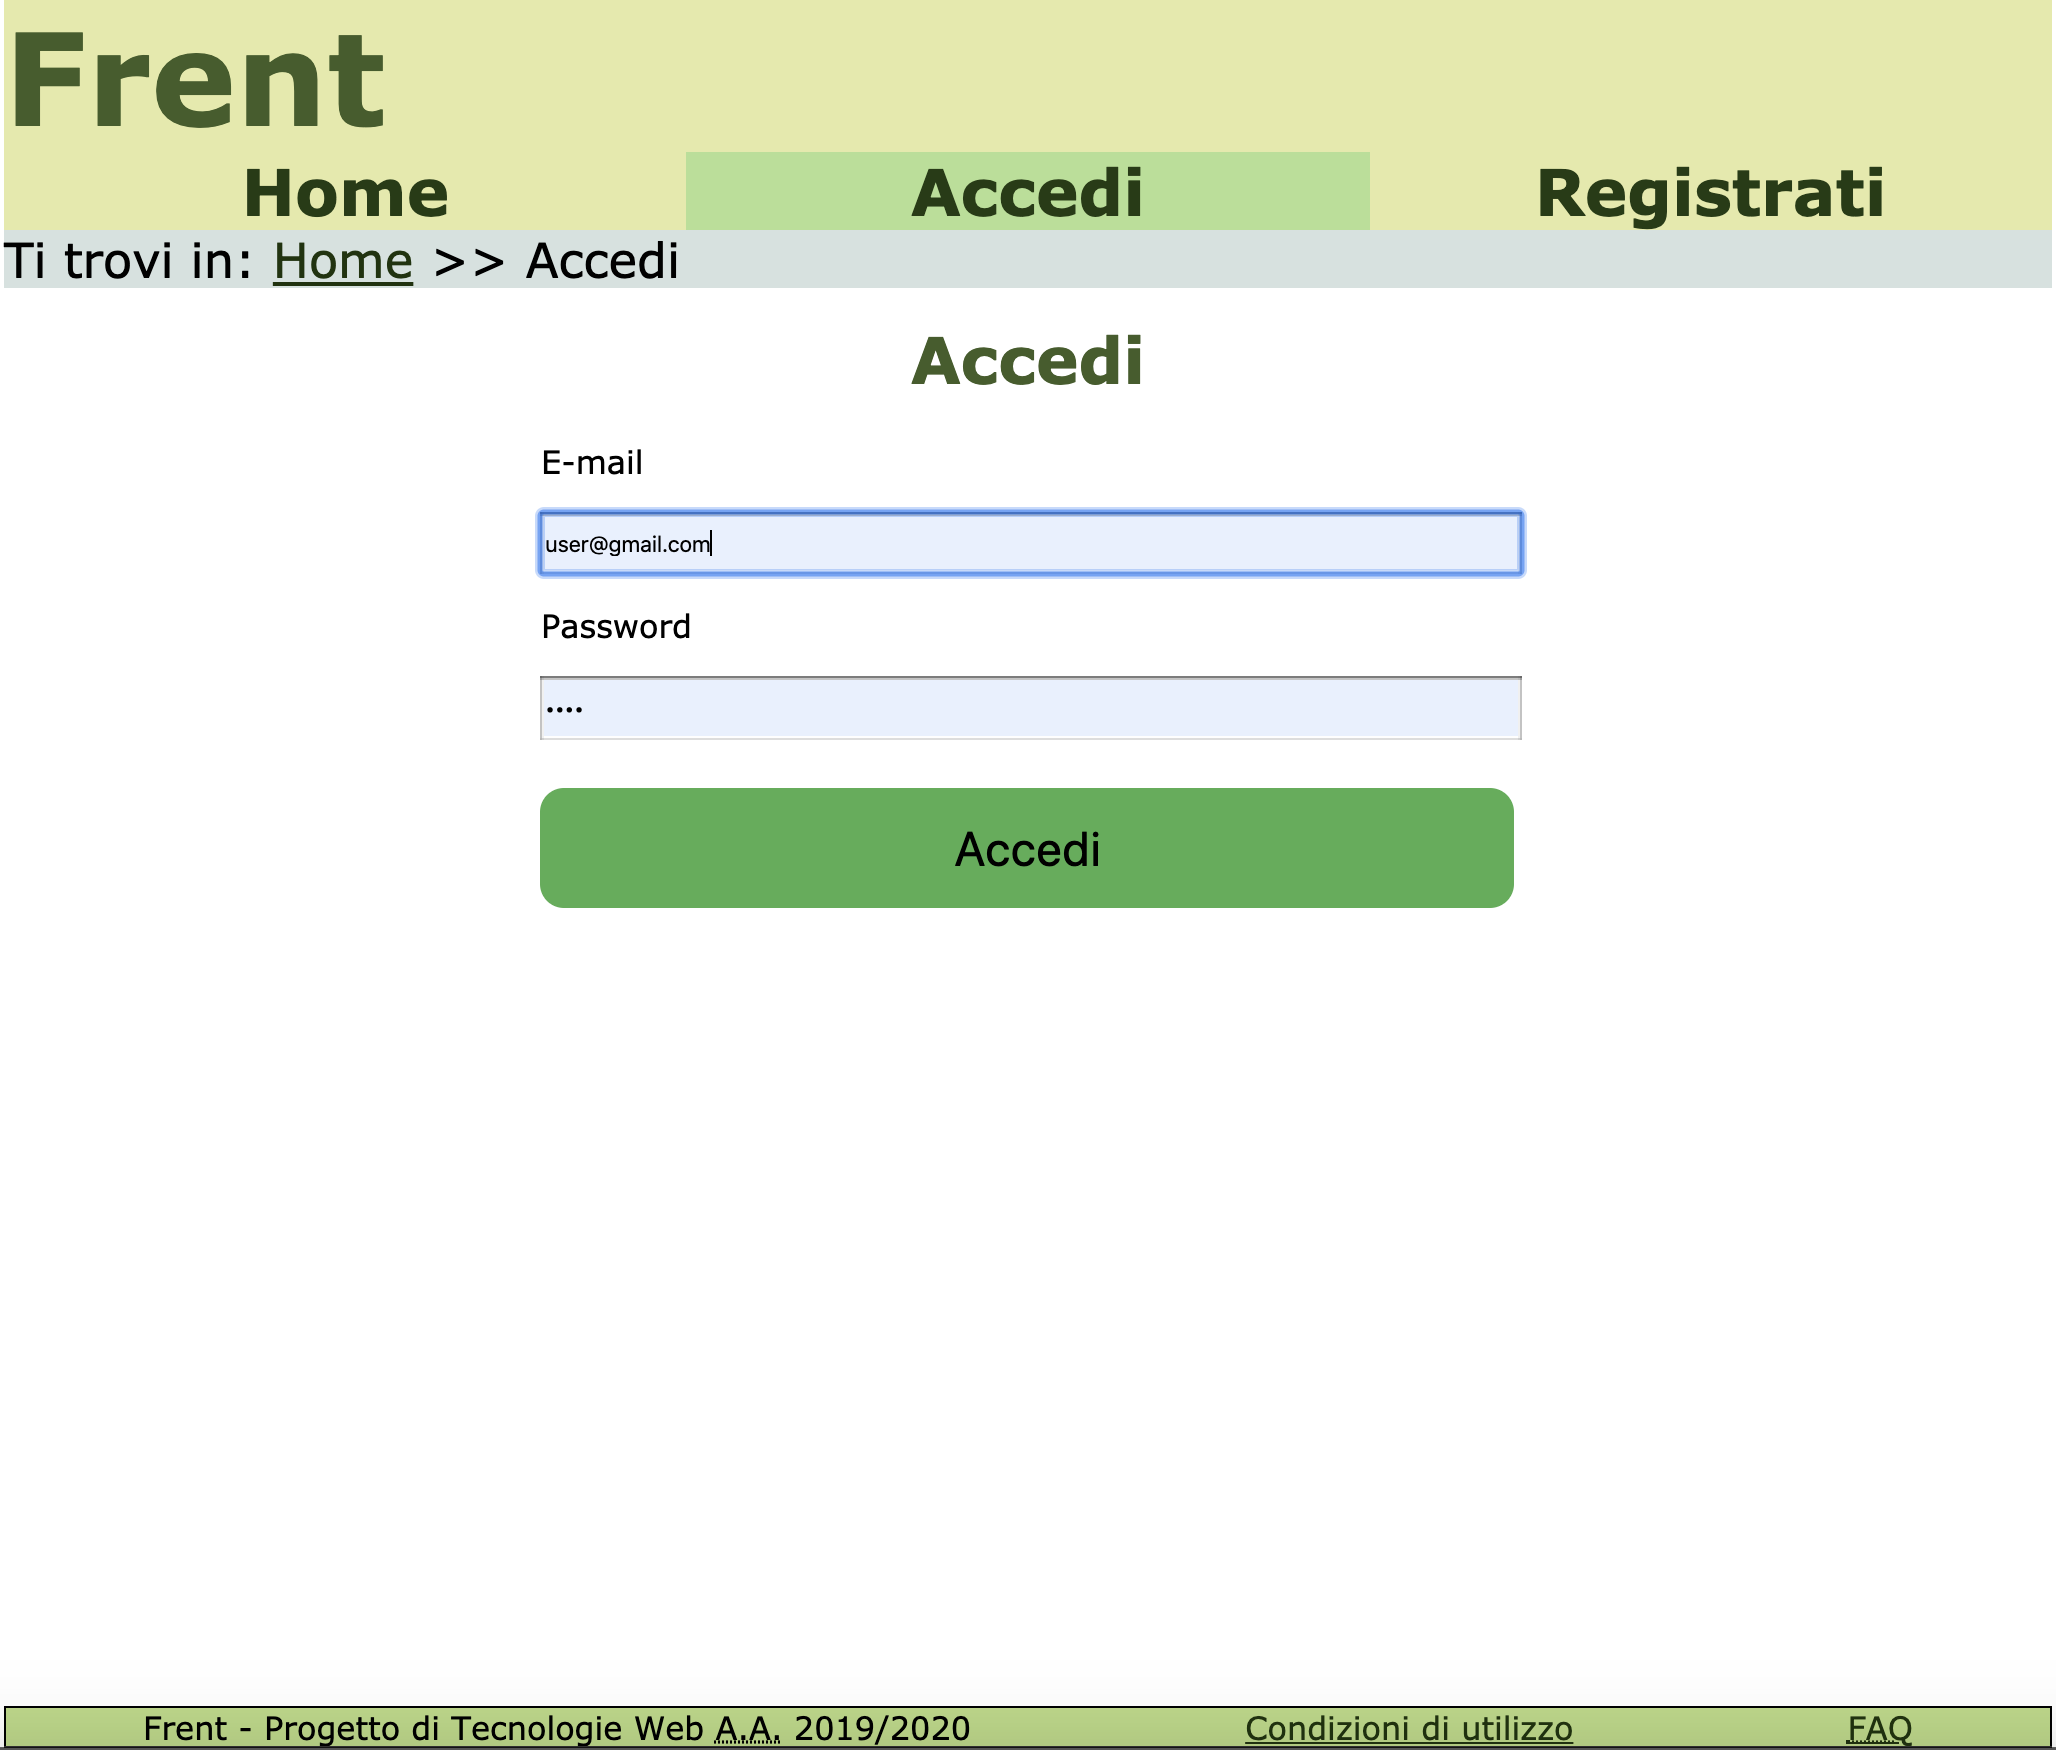
\includegraphics[scale=0.3]{immagini/LayoutCentrale.png}
    \caption{Esmepio di layout centrale}
\end{figure}

\begin{figure}[h!]
    \centering
    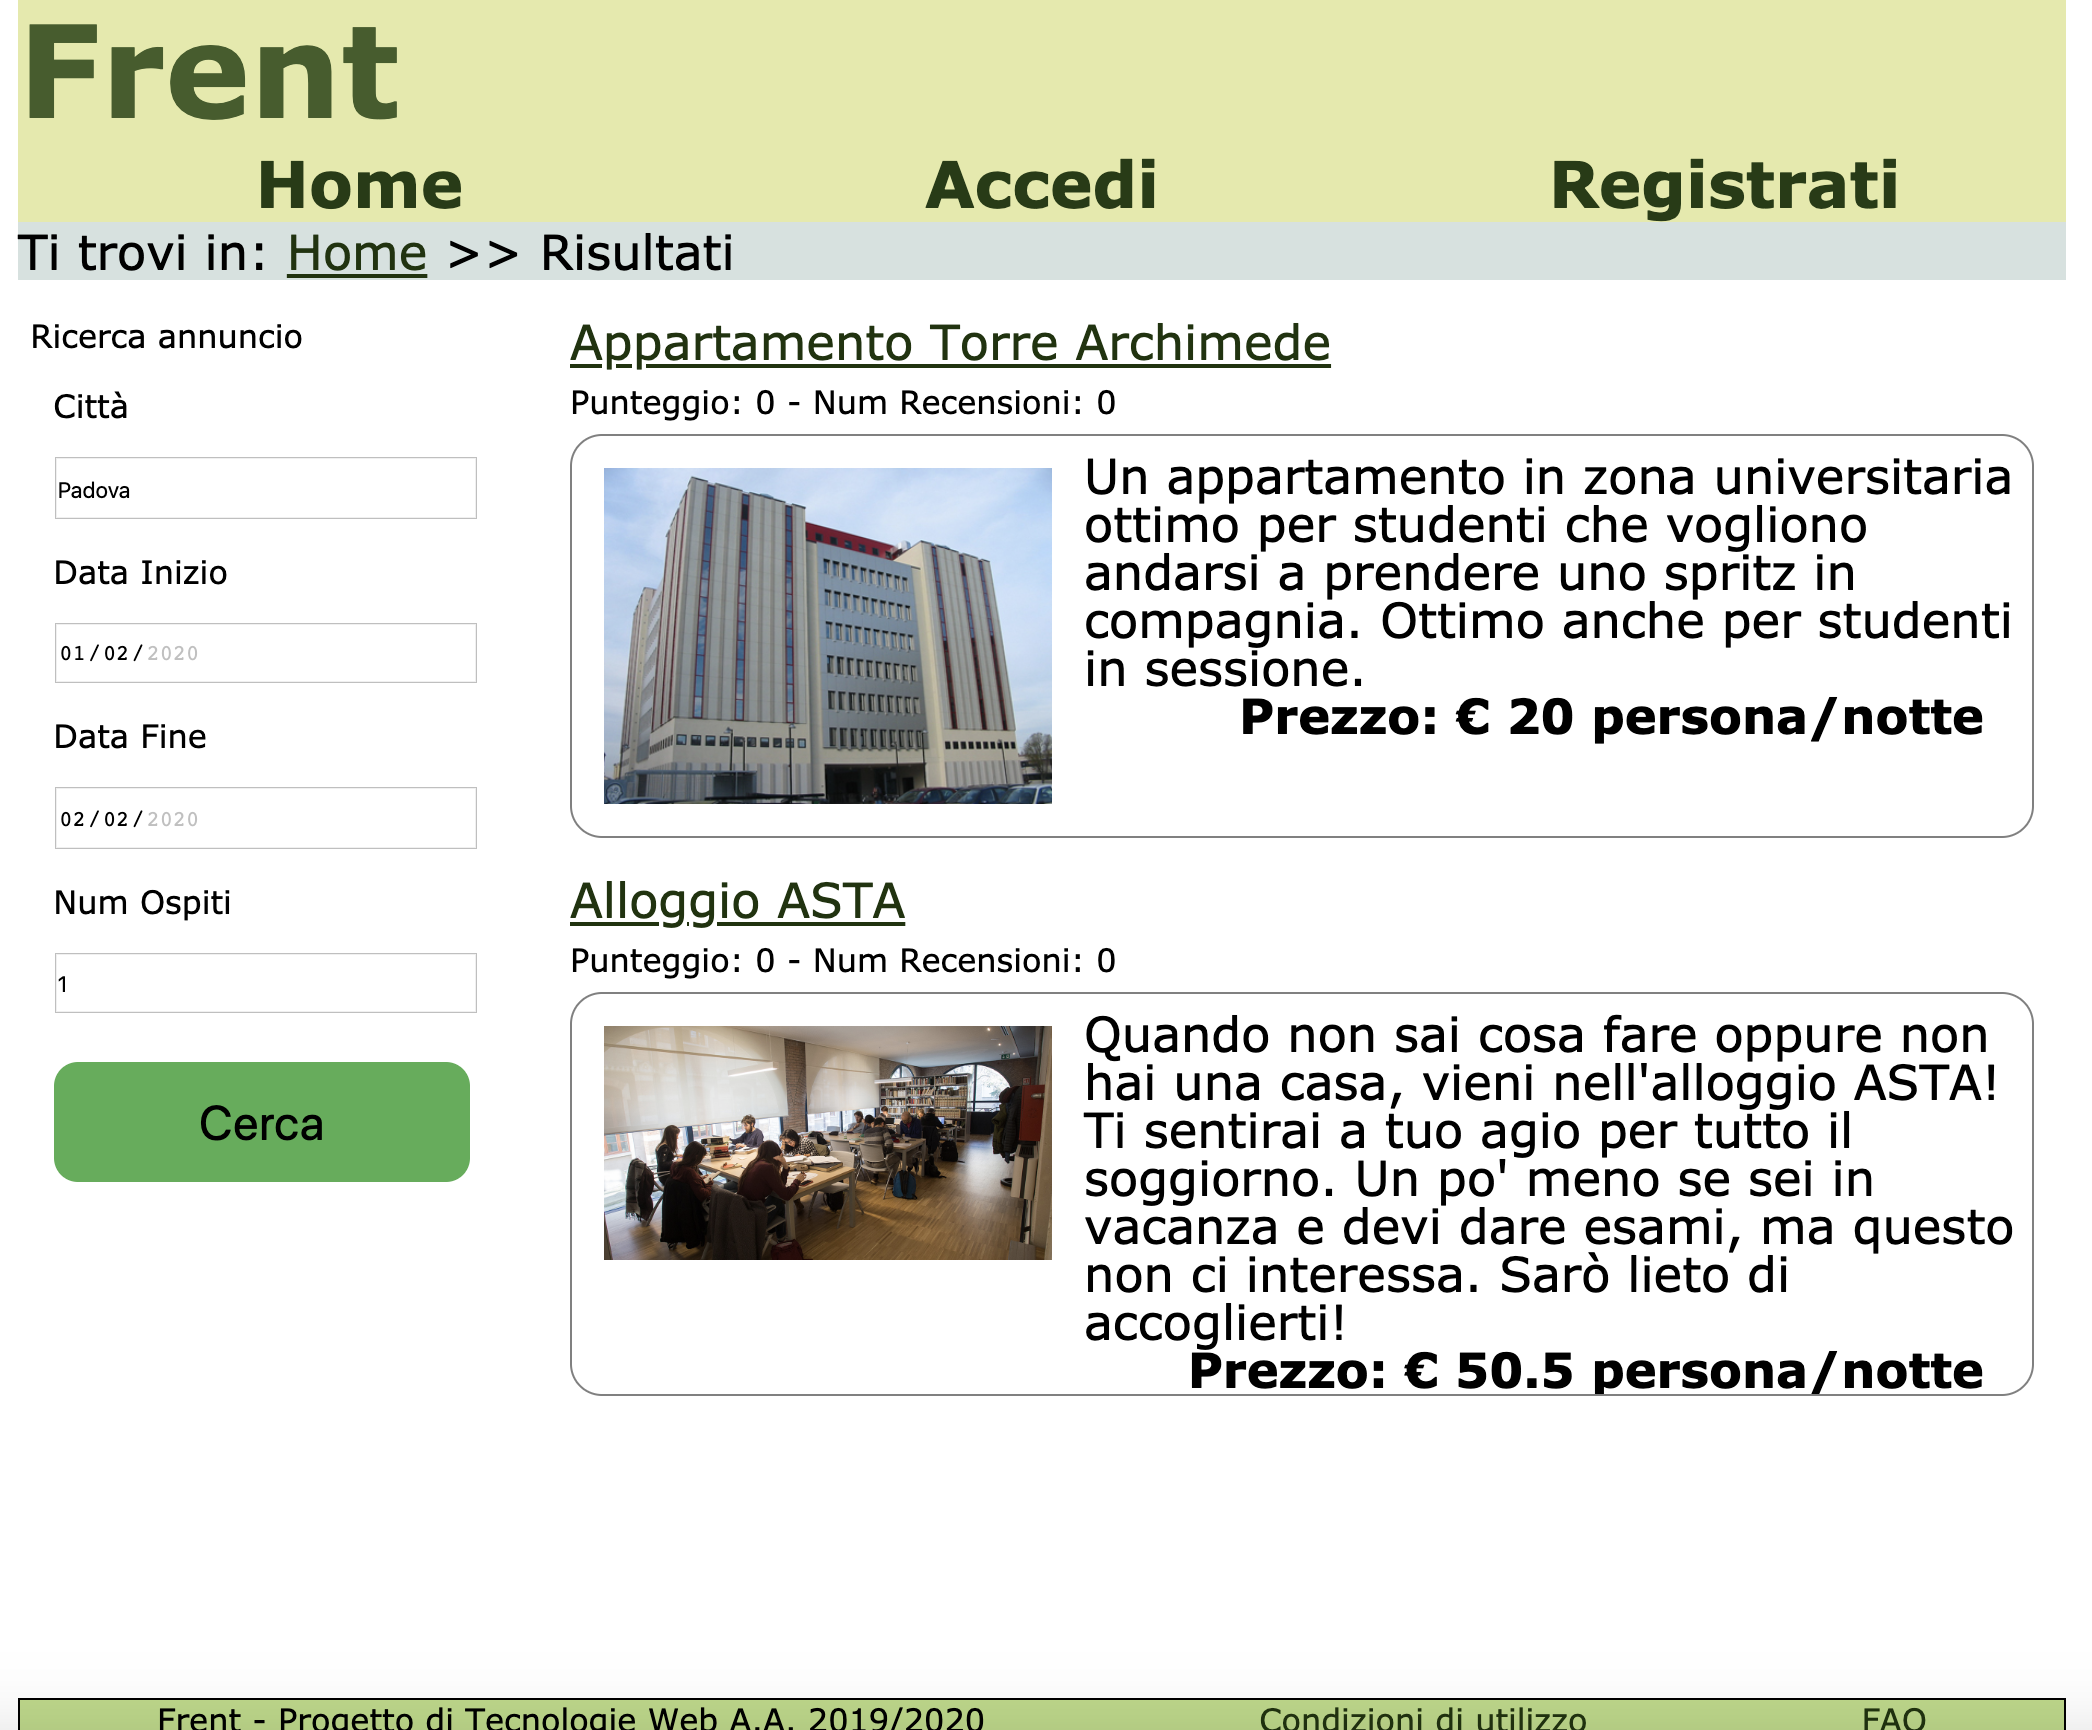
\includegraphics[scale=0.3]{immagini/LayoutTrePannelli.png}
    \caption{Esmepio di layout a tre pannelli}
\end{figure}

\subsubsection{Form}
Tutti i form rispettano le stesse convenzioni interne per non creare disorientamento nell'utente. Per modificare e inserire i dati abbiamo utilizzato dei form posizionati al centro della pagina. Nel momento in cui l'utente modifica i dati non ha bisogno di accedere ad altre tipologie di informazioni all'interno della pagina.\\ Fanno eccezione i form orizzontali e verticali di ricerca annunci che per\`{o} devono essere integrati nella pagina come abbiamo spiegato nella sezione sulla progettazione.

\subsubsection{Scelta dei colori}
Per scegliere i colori abbiamo utilizzato un palette messa a disposizione dalla W3C. La scelta del colore \`{e} stata fatta in modo da evitare possibili problemi di contrasto dopo aver provato diverse combinazioni. Non abbiamo l'esperienza necessaria per poter fare una scelta precisa dei colori. Abbiamo quindi cercato di utilizzare i colori nel modo pi\`{u} semplice possibile per non creare disorientamento all'utente.

\subsubsection{Versione Mobile}
L'interfaccia mobile è stata realizzata principalmente sviluppando su dispositivi reali (Android e iOS) in quanto abbiamo trovato molto poco affidabili gli strumenti offerti dai diversi browser.\\
Sfruttando i grid layout descritti sopra è stato molto semplice riorganizzare i contenuti delle pagine tramite la ridefinizione dell'attributo \textit{gird-template-areas}.\\
Principalmente abbiamo verticalizzato tutti i componenti a partire dagli elementi del menù e del footer; questa scelta è stata fatta per evitare un possibile scroll orizzontale ritenuto molto scomodo per tutti gli utenti del sito.\\

\begin{figure}[h!]
    \centering
    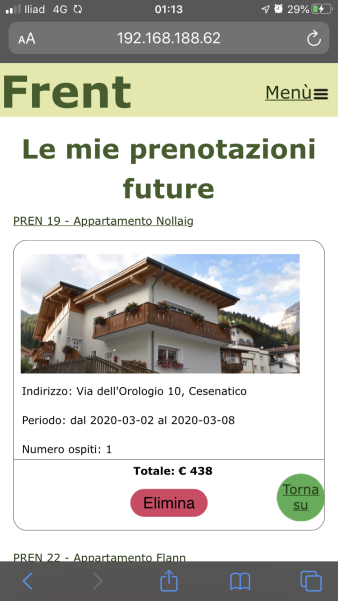
\includegraphics[scale=0.4]{immagini/ricercaMobile.png}
    \caption{Esmepio di ricerca di un annuncio visto da mobile con verticalizzazione degli elementi di una lista}
\end{figure}

\subsubsection{Versione per browser obsoleti}
Siccome facciamo ampio uso del \textit{grid-layout} è sorto il problema della retro-compatibilità con browser che non supportano tale feature di CSS3. Siccome tra i browser che siamo interessati a supportare c'è Internet Explorer 10/11 abbiamo introdotto delle specifiche regole per queste versioni che hanno lo scopo di riorganizzare il contenuto in modo che sia fruibile anche dagli utenti di questo browser.

\subsection{Comportamento}
Per gestire il comportamento del sito abbiamo usato due tecnologie, PHP (lato server) e JavaScript (lato client).

\subsubsection{PHP}
Per rendere il sito dinamico \`{e} stato utilizzato il linguaggio PHP.
La struttura del sistema \`{e} composta da:
\begin{itemize}
    \item Classe \textbf{Database} permette l'apertura e la chiusura di connessioni con il database MySQL realizzato e illustrato nella sezione Progettazione.
    Avendo realizzato una funzione o una procedura SQL per ogni funzionalit\`{a} offerta dal sito, sono presenti due metodi queryProcedure e queryFunction ottimizzati per l'interrogazione del database rispettivamente con procedure e funzioni;
    \item Classe \textbf{Frent} permette di effettuare le chiamate alle procedure o funzioni presenti nel database. Si interfaccia con la classe Database per le interrogazioni e si occupa di controllare gli input inseriti dall'utente e di segnalare violazioni di precondizioni sui dati;
    \item Classi \textbf{Amministratore}, \textbf{Annuncio}, \textbf{Commento}, \textbf{Prenotazione}, \textbf{Utente} sono delle classi che rappresentano le entit\`{a} del database. Contengono metodi set e get per ogni attributo presente nella rispettiva tabella del database e si occupano anche del controllo di validit\`{a} degli input;
    \item Classe \textbf{CredenzialiDB} viene usata per salvare le credenziali di accesso al database MySQL del progetto;
    \item Classe \textbf{DataConstraints} \`{e} una classe di raccolta che viene usata per salvare i limiti di lunghezza dei dati impostati nel database, permettendo cos\`{i} la gestione centralizzata. In questo modo, le eventuali modifiche alla dimensione di un campo di una determinata tabella pu\`{o} essere propagata facilmente a tutto il sito;
    \item Classe \textbf{ImageManager} libreria molto semplice sviluppata per il caricamento dei file immagine (singoli o multipli) da form HTML con salvataggio in una directory scelta dall'utente. Nel nostro progetto, questa directory è \textbf{uploads/};
    \item Classe \textbf{Eccezione} ridefinisce la classe Exception di PHP;
    \item \textbf{Pagine} le pagine PHP vengono create prendendo in input la pagina HTML statica corrispondente, che è stata modificata aggiungendo delle stringhe placeholder, che gli script PHP cercano e sostituiscono con le informazioni che reperiscono dal database.
    Queste pagine non interagiscono direttamente con il database, ma lo fanno chiamando i metodi della classe Frent.
    Questa scelta \`{e} stata presa per tenere separata la struttura (che non cambia), dal comportamento.
    \item \textbf{Script}: sono dei file PHP con al loro interno degli script che ricevono dei dati da elaborare (tipicamente dai form HTML o dalla sessione) per effettuare delle operazioni lato server, senza mostrare direttamente il processo all'utente, ma solo il risultato finale reindirizzando l'utente ad un'altra pagina.
    Esempi di questi script sono quelli per il logout, l'eliminazione di un profilo e il controllo di validità dei dati di una prenotazione.
    \item \textbf{Loader}: sono dei file PHP con al loro interno insiemi di istruzioni che compiono un determinato procedimento.\newline Ne sono stati creati due, uno per il caricamento delle classi fin qui illustrate (\textbf{frent/load\_Frent.php}) e uno per la selezione dell'header da mostrare all'utente (\textbf{frent/load\_header.php}) in base alla pagina in cui si trova e alla categoria di utenza.
\end{itemize}
Le pagine PHP sono state create utilizzando meno possibile il codice HTML nei file PHP.
Ad esempio, nella pagina \textbf{frent/miei\_annunci.php} la definizione della struttura del singolo annuncio \`{e} stata delegata al file \textit{frent/components/item\_mio\_annuncio.html}, così da garantire la separazione della struttura dal comportamento.
L'unico file che non rispetta la separazione in maniera abbastanza importante è il file \textit{frent/load\_header.php}.\\

Si è deciso inoltre di gestire la maggior parte degli errori attraverso il lancio di eccezioni (del tipo Eccezione definito sopra), in quanto questi errori sono tipicamente fatali.
Quando vengono lanciati degli errori dalle chiamate ai metodi delle classi sopra definite, se l'errore:
\begin{itemize}
    \item \`{E} stato causato dall'inserimento errato di un valore, viene mostrato un messaggio di errore;
    \item Se non \`{e} stato causato dall'utente, ma ad esempio da una richiesta al database fallita o di una pagina inesistente, la pagina reagisce in uno dei seguenti modi:
    \begin{enumerate}
        \item L'utente viene re-indirizzato alla pagina \textbf{frent/error\_page.php} con un eventuale messaggio di errore il più possibile esplicativo;
        \item L'utente viene re-indirizzato alla pagina \textbf{frent/404.php};
        \item Interviene il server e mostra l'eventuale errore. In questo particolare caso non è stato possibile per noi (data la configurazione del server ospitante il progetto) modificarne il comportamento.
    \end{enumerate}
\end{itemize}
Quando un utente si registra al sito viene creata di default una cartella \textit{uploads/userID}, con \textit{ID} l'ID dell'utente assegnato all'utente, dove verranno caricati tutti i file da lui aggiunti come immagini profilo (\textit{uploads/userID/imgProfiloID}) e anteprime degli annunci (\textit{uploads/userID/AnnuncioID\_ANNUNCIO}).

\subsubsection{JavaScript}
Il linguaggio JavaScript \`{e} stato impiegato come complemento al sito e non come strumento per implementarne le funzionalità.
Infatti, alcuni utenti potrebbero aver scelto di disabilitare JavaScript all'interno del browser oppure avere un browser obsoleto. Entrambi i casi sono stati considerati da noi molto rari, ma non impossibili.
Per questo motivo abbiamo ridotto al solo essenziale le funzionalità svolte dallo script JavaScript \textbf{frent/form\_validator.js}.
Questo file ha il solo compito di contenere le funzioni che vengono invocate dai form alla pressione del pulsante di submit, le quali si occupano di controllare l'input dell'utente prima dell'invio al server (ovvero all'esecuzione di codice PHP).
Le funzioni chiamate dai form HTML sono quelle con il nome che comincia con \textit{validazione\_form}. Saranno queste funzioni a richiamare le singole funzioni, \textit{check\_nome\_campo}, per controllare la validit\`{a} dei valori inseriti dall'utente.
Se il controllo effettuato ha successo viene restituito \textbf{true}, altrimenti viene visualizzato un messaggio di errore informativo implementato con un elemento \textit{strong} e successivamente restituito \textbf{false}.

\subsection{Indicizzazione}
Abbiamo aggiunto il file robots.txt per indicare agli user agent (i motori di ricerca) quali pagine non indicizzare. In pratica, tutte le pagine accessibili al sono utente registrato non vengono indicizzate. Il motore di ricerca, provando ad accedervi, troverebbe solo la pagina di login (o di errore in base a come viene gestito) quindi sarebbe inutile permetterne l'indicizzazione.
\end{document}